\usetikzlibrary {circuits.logic.US}
\usetikzlibrary {calc}
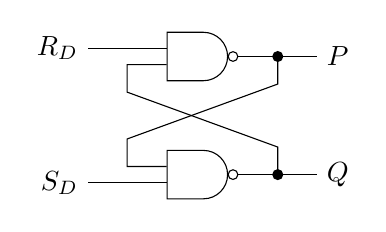
\begin{tikzpicture}[circuit logic US]
  % draw NAND gate 1
  \draw (0,1.5) node[nand gate,inputs={nn}] (nand1) {};
  
  % draw NAND gate 2
  \draw (0,0) node[nand gate,inputs={nn}] (nand2) {};

  % draw flip-flop
  \draw (nand1.output) -- ++(right:1);
  \draw (nand2.output) -- ++(right:1);
  \draw (nand1.input 1) -- ++(left:1);
  \draw (nand2.input 2) -- ++(left:1);

  \draw (nand2.input 1) -- ++(left:0.5) -- ++(up: 0.35)
        -- ($(nand1.output) + (0.5, -0.35)$)
        -- ($(nand1.output) + (0.5, 0)$);
  \fill ($(nand1.output) + (0.5, 0)$) circle (2pt);

  \draw (nand1.input 2) -- ++(left:0.5) -- ++(down: 0.35)
        -- ($(nand2.output) + (0.5, 0.35)$)
        -- ($(nand2.output) + (0.5, 0)$);
  \fill ($(nand2.output) + (0.5, 0)$) circle (2pt);

  % Draw Labels

  \draw ($(nand2.input 2) +(-1, 0)$) node[left] {$S_D$};
  \draw ($(nand1.input 1) +(-1, 0)$) node[left] {$R_D$};
  \draw ($(nand2.output) +(1, 0)$) node[right] {$Q$};
  \draw ($(nand1.output) +(1, 0)$) node[right] {$P$};
\end{tikzpicture}
